% !TEX root = ./Vorlesungsmitschrift AGLA 2.tex  
\lecture{Fr 21.05. 10:15}{}
Eine Weitere Eignenschaft von Ähnlichkeiten:
\begin{satz}
  Sei \( X \) ein euklidischer affiner Raum und \( f\maps X\to X \) eine Ähnlichkeit mit Ähnlichkeitsfaktor \( \rho\neq 1 \). Dann besitzt \( f \) genau einen Fixpunkt.
\end{satz}
\begin{proof}[Beweisidee]
  Nach obigem Korollar ist \( f \) eine Affinität. Sei \( F\maps T(X)\to T(X) \) die zugehörige lineare Abbildung. Dann ist \( \frac{1}{\rho} F \) orthogonal, also haben alle Eigenwerte von \( F \) Betrag \( \rho \). 

  Nach Wahl eines Koordinatensystem wird \( f \) beschrieben durch
  \begin{align*}
    \reals^n&\to \reals^n\\
    x&\mapsto \braceannotate{\isittrue{=}x}{Ax+b}.
  \end{align*}
  mit \( A\in \sqmatrices{n}{\reals} \), \( k\subset \reals^n \) und Fixpunkten beschrieben durch
  \begin{equation*}
    Ax+b=x,
  \end{equation*}
  also \( (A-I_n)x=-b \), da \( 1 \) kin Eigenwert von \( A \) ist, gilt \( \det(A-I_n)\neq 0 \).
\end{proof}
Ähnlichkeiten erhalten Winkel. Gibt es noch weitere Affinitäten eines euklidischen affinen Raumes, die Winkel erhalten?
\begin{definition*}
  Sei \( X \) ein euklidischer affiner Raum, \( L,L'\subseteq X \) Geraden mit \( L\cap L'\neq \emptyset \). Wir nennen \( L \) und \( L' \) orthogonal, wenn gilt
  \begin{equation*}
    \lineangle{L}{L'}=\frac{\pi}{2}.
  \end{equation*}
  Schriebe auch \( L\perp L' \).
\end{definition*}
\begin{satz}\label{nur_aehnlichkeiten_erhalten_rechte_winkel}
  Sei \( X \) ein euklidischer affiner Raum und \( f\maps X\to X \) eine Affinität mit der Eigenschaft, dass für alle Geraden \( L,L' \) mit \( L\cap L'\neq \emptyset \) und \( L\perp L' \) gilt, dass
  \begin{equation*}
    f(L)\perp f(L').
  \end{equation*}
  Dann ist \( f \) eine Ähnlichkeit.
  \begin{figure}[H]
    \centering
    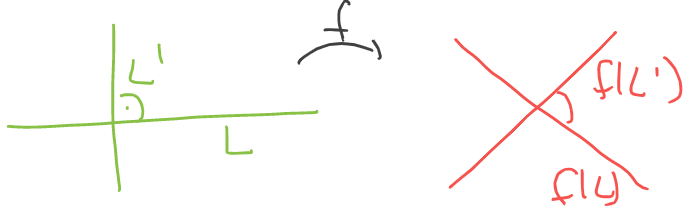
\includegraphics[width=0.5\linewidth]{figures/rechte_winkel_erhalten}
    \label{fig:rechte_winkel_erhalten}
  \end{figure}
\end{satz}
\begin{proof}
  Sei \( F\maps T(X)\to T(X) \) die zugehörige bijektive lineare Abbildung. Seien \( p,q,q'\in X \) mit \( p\vee q=L \), \( p\vee q'=L' \) und \( L\perp L' \). Dann gilt \( \lineangle{L}{L'}=\frac{\pi}{2} \), also
  \begin{equation*}
    \arccos \frac{\abs{\scalarproduct{\vv{pq}}{\vv{pq'}}}}{\norm{\vv{pq}}\norm{\vv{pq'}}}=\frac{\pi}{2}
  \end{equation*}
  \dh \( \scalarproduct{\vv{pq}}{\vv{pq'}}=0 \).
  \begin{figure}[H]
    \centering
    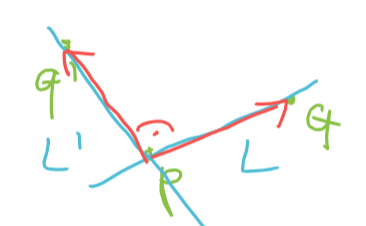
\includegraphics[width=0.5\linewidth]{figures/rechte_winkel_skalarprodukt}
    \label{fig:rechte_winkel_skalarprodukt}
  \end{figure}
  Die Geraden \( f(L) \) und \( f(L') \) sind gegeben durch
  \begin{equation*}
    f(p)\vee f(q)=f(L)\qquad f(p)\vee f(q')=f(L')
  \end{equation*}
  und wir können annehmen (wegen \( f(L)\perp f(L') \)), dass 
  \begin{equation*}
    \braceannotate{\scalarproduct{F(\underrelate{\vertni}{T(X)}{\underbrace{\vv{pq}}})}{F(\underrelate{\vertni}{T(X)}{\underbrace{\vv{pq'}}})}}{\scalarproduct{\vv{f(p)f(q)}}{\vv{f(p)f(q')}}}=0.
  \end{equation*}
Es gilt also, dass für alle \( v,w\in T(X) \) mit \( \scalarproduct{v}{w}=0 \) gilt \( \scalarproduct{F(v)}{F(w)}=0 \). Wir haben den Beweis von \thref{nur_aehnlichkeiten_erhalten_rechte_winkel} auf folgendes Lemma reduziert.
\end{proof}
\begin{lemma}
  Sei \( V \) ein euklidischer Vektorraum, \( F\maps V\to V  \) ein Isomorphismus mit \( F(v)\perp F(w) \) für alle \( v,w\in V \) mit \( v\perp w \). Dann existiert \( \rho\in \reals_{>0} \) \sd \( \frac{1}{\rho}\cdot F \) orthogonal ist.
\end{lemma}
\begin{proof}
  Sei \( n=\dim-{V} \) und \( v_1,\dotsc, v_n \) eine Orthonormalbasis von \( V \), \dh \( \norm{v_i}=1 \), \( 1\leq i\leq n \) und \( \scalarproduct{v_i}{v_\gamma}=0 \) für \( i\neq j \). Sei \( \rho_i\definedas \norm{F(v_i)}  \), \( 1\leq i \leq n \).
  \begin{figure}[H]
    \centering
    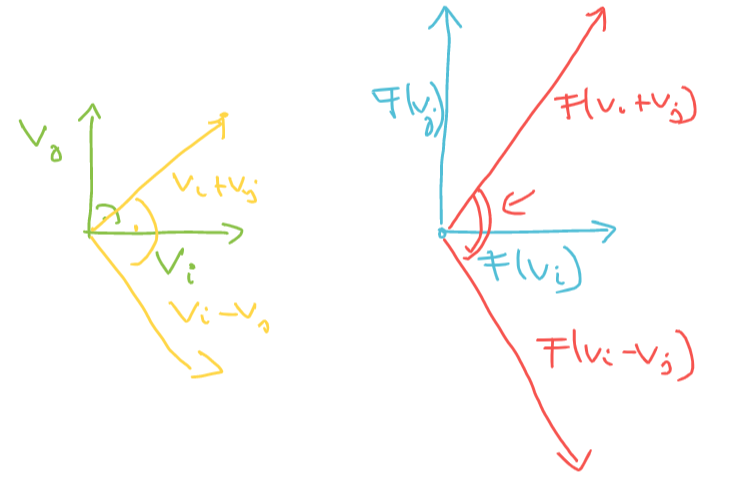
\includegraphics[width=0.5\linewidth]{figures/orthonormalbasis_skalierung}
    \label{fig:orthonormalbasis_skalierung}
  \end{figure}
  Fpr \( i\neq j \) gilt 
  \begin{equation*}
    \scalarproduct{v_i+v_j}{v_i-v_j}=\braceannotate{=1}{\norm{v_i}^2}+\braceannotate{=0}{\scalarproduct{v_j}{v_i}}-\braceannotate{=0}{\scalarproduct{v_i}{v_j}}-\braceannotate{=1}{\norm{v_j}^2}=0, 
  \end{equation*}
  also \( v_i+v_j\perp v_i-v_j \). Nach Annahme gilt dann auch
  \begin{align*}
    \scalarproduct{F(v_i)}{F(v_i)}+\braceannotate{=0, \text{ da } F(v_j)\perp F(v_i)}{\scalarproduct{F(v_j)}{F(v_i)}}-\braceannotate{=0}{\scalarproduct{F(v_i)}{F(v_j)}}-\scalarproduct{F(v_j)}{F(v_j)}&=\scalarproduct{F(v_i+v_j)}{F(v_i-v_j)}\\
    &=0.
  \end{align*}
  Also gilt
  \begin{equation*}
    \equalto{\rho_i^2}{\norm{F(v_i)}^2}=\equalto{\rho_j^2}{\norm{F(v_j)}^2} \quad \forall i,j
  \end{equation*}
  und damit \( \rho_i=\rho_j \quad \forall 1\leq i,j\leq n \). Schreibe \( \rho=\rho_i \quad \forall 1\leq i \leq n \) für den gemeinsamen Wert. Dann ist die Abbildung \( \frac{1}{\rho}F \) orthogonal, da \( v_1,\dotsc, v_n \) auf die Orthonormalbasis \( \frac{1}{\rho}F(v_1),\dotsc,\frac{1}{\rho}F(v_n) \) abgebildet wird.
\end{proof}
Sei \( f\maps \reals^n\to \reals^n \) eine Affinität gegeben durch 
\begin{equation*}
  x\mapsto Ax+b\qquad A\in \invertiblematrices{n}{\reals}\quad b\in \reals^n.
\end{equation*}
Im Obigen haben wir gesehen, dass gilt: \( f \) ist \emph{Kongruenz} \tiff \( A \) ist \emph{orthogonal}, \( f \) ist Ähnlichkeit \( \frac{1}{\rho}A \) ist orthogonal für ein \( \rho\geq 0 \).
\begin{frage*}
  Wie können wir \( A\in \invertiblematrices{n}{\reals} \) für eine allgemeine Affinität \( f \) mit Hilfe von / bis auf eine orthogonale Matrix möglichst einfach ausdrücken?
\end{frage*}
\file{Hauptachsentransformation Affinitäten}
Betrachte \( \reals^n \) als euklidischen affinen Raum mit Standardskalarprodukt
\begin{gather*}
  \scalarproduct{\cdot}{\cdot}\maps \begin{aligned}[t]
    \reals^n\times\reals^n &\to \reals_{\geq 0}\\
    (x_1,\dotsc,x_n)\times(y_1,\dotsc,y_n)&\mapsto \sum_{i=1}^{n}x_i y_i.
  \end{aligned}
\end{gather*}
\begin{satz}[Hauptachsentransformation von Affinitäten]\label{hauptachsentransformation_affinitaeten}
  Sei \( f\maps \reals^n\to \reals^n \) eine Affinität gegeben durch \( x\mapsto Ax+b \) mit \( A\in \invertiblematrices{n}{\reals} \), \( b\in \reals^n \). Dann gibt es orthogonale Matrizen \( S,T\in \orthogonalmatrices{n} \) und eine Diagonalmatrix
  \begin{equation*}
    D=\begin{pNiceMatrix}
      \alpha_1 &  & \Block{2-2}<\large>{0} & \\
       & \alpha_2 & & \\
      \Block{2-2}<\large>{0} &  & \Ddots \\
       &  & & \alpha_n
    \end{pNiceMatrix}
  \end{equation*}
  mit \( \alpha_1,\dotsc,\alpha_n>0 \), \sd
  \begin{equation*}
    A=SDT
  \end{equation*}
  \dh
  \begin{equation*}
    f(x)=SDTx+f(0).
  \end{equation*}
\end{satz}
\begin{proof}
  Wir bilden die Matrix \( C=\transpose{A}A \).
  \begin{itemize}
    \item \( C \) ist symmetrisch, da
    \begin{equation*}
      \transpose{C}=\transpose+{\transpose{A}A}=\transpose{A}\transpose{\transpose{A}}=\transpose{A}A=C.
    \end{equation*}
    \item \( C \) ist positiv definit, denn \( I_n \) ist positiv definit und daher nach dem Sylvesterschen Trägheitsgesetz auch \( C \). Aus der Hauptachsentransformation symmetrischer Matrizen (\aglacourse{1}) folgt, dass es eine Matrix \( T\in \orthogonalmatrices{n} \) mit
    \begin{equation*}
      TC\transpose{T}=\begin{pNiceMatrix}
        \beta_1 &  & 0 \\
         & \Ddots &  \\
        0 &  & \beta_n
      \end{pNiceMatrix},
    \end{equation*}
    \( \beta_1,\dotsc,\beta_n>0 \). Wir definieren \( \alpha_i=\sqrt{\beta_i} \), \( 1\leq i\leq n \) und 
    \begin{equation*}
      D\definedas \begin{pNiceMatrix} \alpha_1 &  &  \\  & \Ddots &  \\  &  & \alpha_n \end{pNiceMatrix},
    \end{equation*}
    Dann gilt
    \begin{equation*}
      T\braceannotate{\transpose{A}A}{C}\transpose{T}=D^2=\transpose{D}D,
    \end{equation*}
    also
    \begin{equation*}
      I_n=\braceannotate{S}{\inv{\transpose{A}}\transpose{T}\transpose{D}}\braceannotate{\transpose{S}}{DT\inv{A}}.
    \end{equation*}
    Sei \( S\definedas \inv{\transpose{A}}\transpose{T}\transpose{D} \). Dann gilt \( \transpose{S}S=I_n \) und \( S\in \orthogonalmatrices{n} \) ist orthogonal. Wir erhalten \( \transpose{S}=DT\inv{A} \) und \( A=SDT \).
  \end{itemize}
\end{proof}
\begin{korollar*}
  Sei \( f\maps \reals^n\to \reals^n \) ein Isomorphismus des Vektorraumes \( \reals^n \). Dann gibt es eine Orthonormalbasis \( v_1,\dotsc, v_n\in \reals^n \), \sd die Vektoren \( F(v_1),\dotsc,F(v_n) \) eine Orthogonalbasis bilden.
\end{korollar*}
\begin{proof}
  Sei \( F \) bezüglich der Standardbasis der \( \reals^n \) gegeben durch die Matrix \( A\in \invertiblematrices{n}{\reals} \). Aus \thref{hauptachsentransformation_affinitaeten} folgt, dass es orthogonale Matrizen \( S,T\in \orthogonalmatrices{n} \) gibt mit \( A=SDT \) und
  \begin{equation*}
    D=\begin{pNiceMatrix}
      \alpha_1 &  & 0 \\
       & \Ddots &  \\
      0 &  & \alpha_n
    \end{pNiceMatrix},
  \end{equation*}
  \( \alpha_1,\dotsc,\alpha_n>0 \) einer Diagonalmatrix. Sei \( v_i=\transpose{T}e_i \), \( 1\leq i\leq n \). \( T \) ist orthogonal, also auch \( \transpose{T} \) und damit ist \( v_1,\dotsc,v_n \) eine Orthonormalbasis des \( \reals^n \). Es gilt
  \begin{align*}
    F(v_i)&=A\transpose{T}e_i\\
    &=SD\braceannotate{T\transpose{T}}{I_n}e_i\\
    &=SDe_i=S(\alpha_i e_i)\\
    &=\alpha_i S_{e_i}.
  \end{align*}
  Die Matrix \( S \) ist orthogonal, also sind die Vektoren \( Se_1,\dotsc,Se_n \) eine Orthonormalbasis. Da \( \alpha_1,\dotsc,\alpha_n>0 \), bilden \( F(v_1),\dotsc,F(v_n) \) eine orthogonal Basis der \( \reals^n \).
\end{proof}
\begin{beispiel*}
  \phantom{Ein Beispiel}
  \begin{figure}[H]
    \centering
    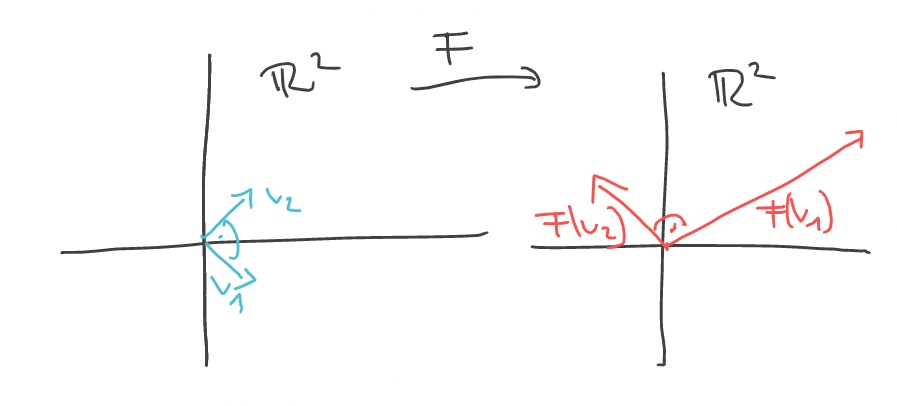
\includegraphics[width=0.5\linewidth]{figures/orthonormalbasis_auf_orthogonalbasis}
    \label{fig:orthonormalbasis_auf_orthogonalbasis}
  \end{figure}
\end{beispiel*}